\setcounter{secnumdepth}{-1}

\chapter{Transmission chain blocks}

\section{Baseband representation}

By looking at the block diagram of the transmission chain \ref{fig:blockDiagram}, one can see we never move the baseband signal to the carrier frequency. As the simulation runs on a computer, using the bandpass representation of the signal would require much more samples as the sampling frequency would need to be at least twice the carrier frequency. By simulating the chain in baseband, the minimal sampling frequency is reduced to the symbol rate in order to have at least one sample per symbol. \\
Because the signal is oversampled, the sampling frequency is then equal to the symbol rate multiplied by the oversampling factor. \\

\section{Modulation and Demodulation}

After generating N random bits, they are modulated. This allows to send fewer symbols than the number of bits. We chose QAM modulation as it combines ASK and PSK. Depending on the number of bits per symbol ($N_{\text{bps}}$), the number of bits sent ($N$) had to be chosen such that  $N / N_{\text{bps}} \in \mathbb{N}$. \\
Figure \ref{fig:QAMComparison} compares the modulation the constellation diagrams obtained for QAM-16 and QAM-64. As the constellations points are more spaced on the left, QAM-16 is less prone to a wrong demodulation (when noise will be added). This comes at the cost of a lower bitrate: for the same symbol rate, QAM-64 will send 6 bits while QAM-16 only send 4. It clearly shows a compromise between reliability and capacity. \\

\begin{figure}[H]
    \centering
    \begin{subfigure}[b]{0.45\linewidth}
        \centering
        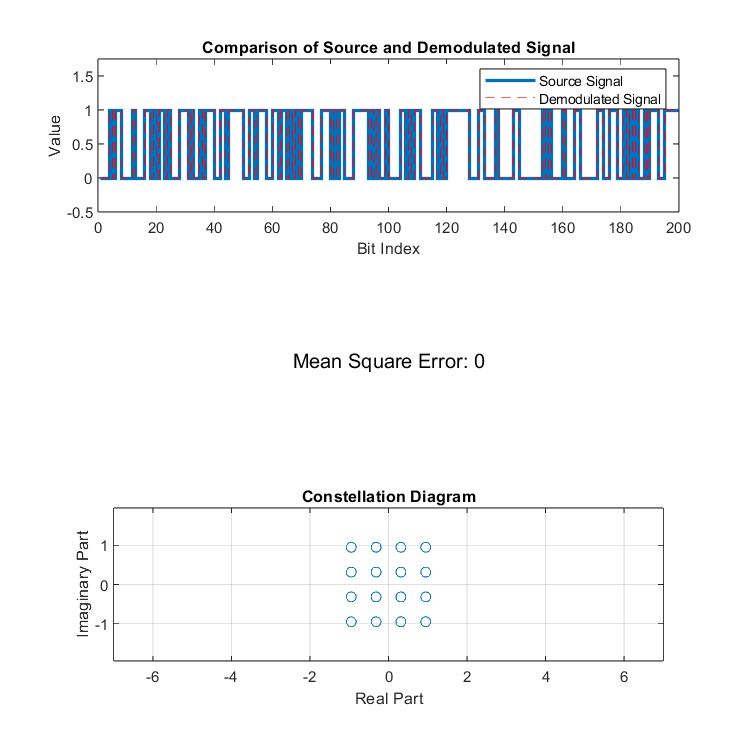
\includegraphics[width=\linewidth]{modulation16.png}
        \caption{QAM-16 modulation}
        \label{fig:QAM16}
    \end{subfigure}
    \hfill
    \begin{subfigure}[b]{0.45\linewidth}
        \centering
        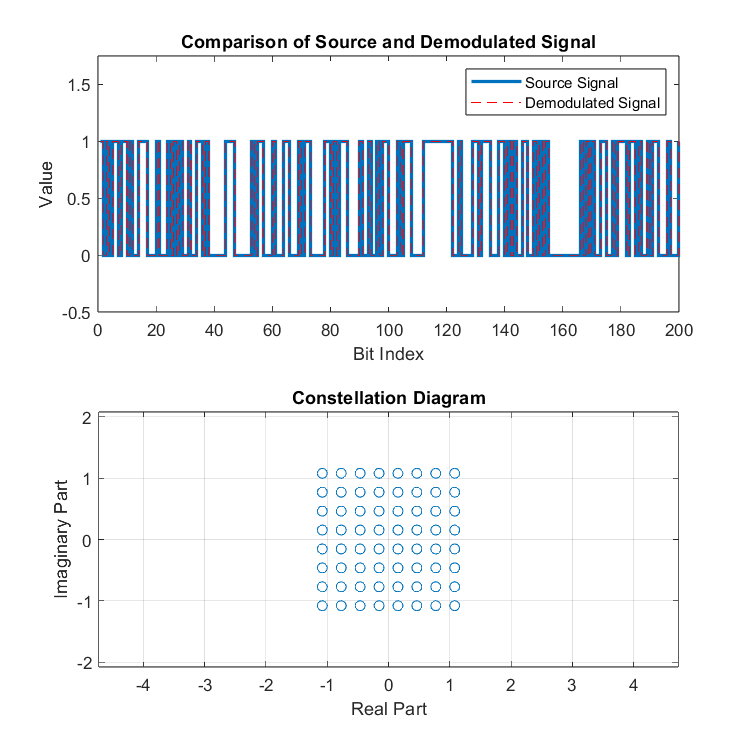
\includegraphics[width=\linewidth]{modulation64.png}
        \caption{QAM-64 modulation}
        \label{fig:QAM64}
    \end{subfigure}
    \caption{Comparison of QAM modulations, where the mean square error is computed between the transmitted and received bitstream}
    \label{fig:QAMComparison}
\end{figure}

\section{Optimal demodulator and detector}

First, it is important to remind that the transmitted signal is characterised / represented by a set of coefficients which results from the projection
 of the signal on the adequate orthonormal basis function related to the choosen modulation.
 Once transmitted, the signal is affected by noise (in our case AWGN noise).  In the general case, this noise reoriante the signal representation outside of the sub-space set during the modulation phase.
To construct an optimal demodulator, 2 criteria should be taken into account.  The first one is the sufficient statistic criteria.  It is proven that once the received signal
is projected on the sub-space defined by the previous basis functions, the noise component outside of the sub-space is indepedent from the projected signal.
It means that we loose no information by projecting the received signal on the original sub-space and we can therefore make an optimal decision based on projected signal.
(based on the coefficient of the projected received signal).

\begin{figure}[H]
    \centering
    \includegraphics[scale = 0.7]{Bank_correlator.png}
    \caption{Projection on basis sub-space}
    \label{fig:Bank_correlator}
\end{figure}

\begin{figure}[H]
    \centering
    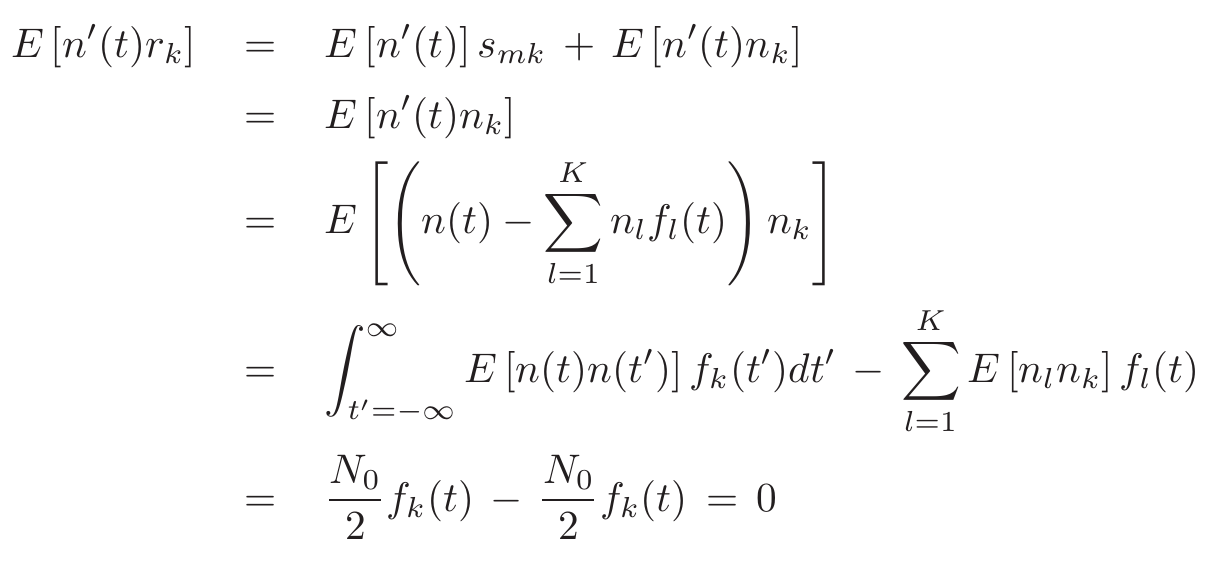
\includegraphics[scale = 0.5]{SufficientStatistic.png}
    \caption{Criteria of sufficient statistics}
    \label{fig:Sufficientstatistic}
\end{figure}

The second criteria is the usage of matched filters. The demodulator used to achieve the sufficient statistic property is composed of bank of correlators (projection of basis function).
Instead of using a bank of correlator, we can use a bank of filters matched to the used basis functions.  It is proven that such filters at the demodulator results to
 a maximized SNR (minimize the power of the noise at the exit of the demodulator).
In conclusion, by using a bank of filters matched on the orthonormal basis function set by the choice of the modulation, we cna construct a optimal demodulator which
 would ensure an optimal decision based on the received signal and ensure a maximum SNR at the output of this demodulator.

 \begin{figure}[H]
    \centering
    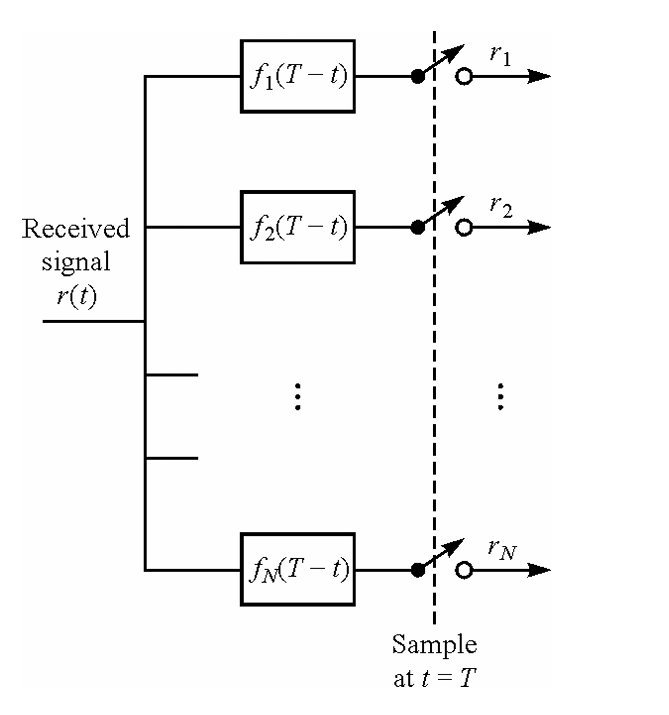
\includegraphics[scale = 0.6]{Matchedfilters.png}
    \caption{Bank of filters matching basis functions}
    \label{fig:Matchedfilters}
\end{figure}

\begin{figure}[H]
    \centering
    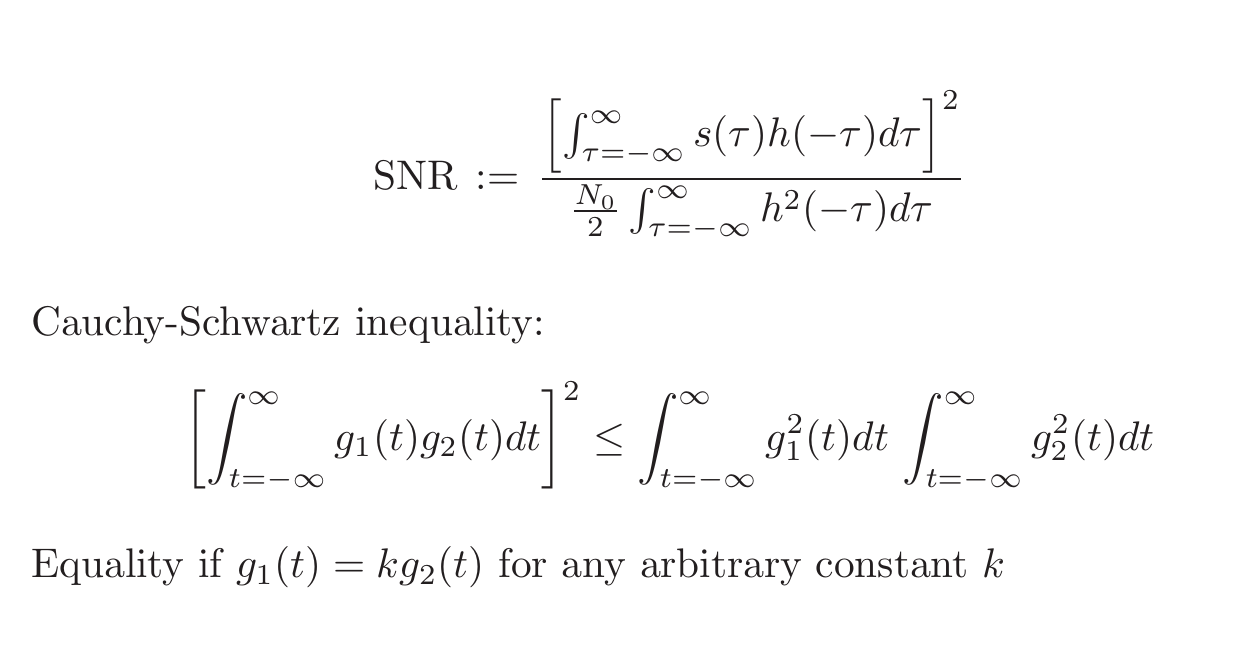
\includegraphics[scale = 0.5]{MaxSNR.png}
    \caption{Maximum SNR demonstration}
    \label{fig:MaxSNR}
\end{figure}

At the output of the demodulator, we still need to ensure to make the optimal choice of the M possible sm(t) based on the received signal.
For that, we would need to follow the maximum likelihood criteria which "decoule" from the maximum a posteriori criteria (general criteria) if each possible sm(t) 
owns the same probability.
The criteria leads to the following result : the optimizal sm(t) choice is found by taking the minimum euclidian distance between the observable received signal r(t) 
and all the possible modulated signal sm(t).

\section{Pulse shaping}

With modulation only, the bandwidth of the transmitted signal is infinite. This is problematic as it could interfere with neighboring channels. A filtering is applied to resolve this but the chosen filter must respect two other constraints: it must cancel inter-symbol interference (ISI) and must maximize the SNR. \\
The raised cosine filter is chosen as it limits the bandwidth and cancels ISI. To maximize the SNR, it is applied as a matched filter by using the square root of it at the transmitter and at the receiver. \\
The time domain and frequency domain representation of the raised cosine filter is shown in Figure \ref{fig:raisedCosine}. Figure \ref{fig:pulseShaping} shows how the signal is shaped in the time domain and how there is indeed no ISI. Finally, the spectrum of the transmitted signal is plotted in figure \ref{fig:shapedSpectrum} where the frequency band is limited to $[-3, 3]$MHz. \\

\begin{figure}[H]
    \centering
    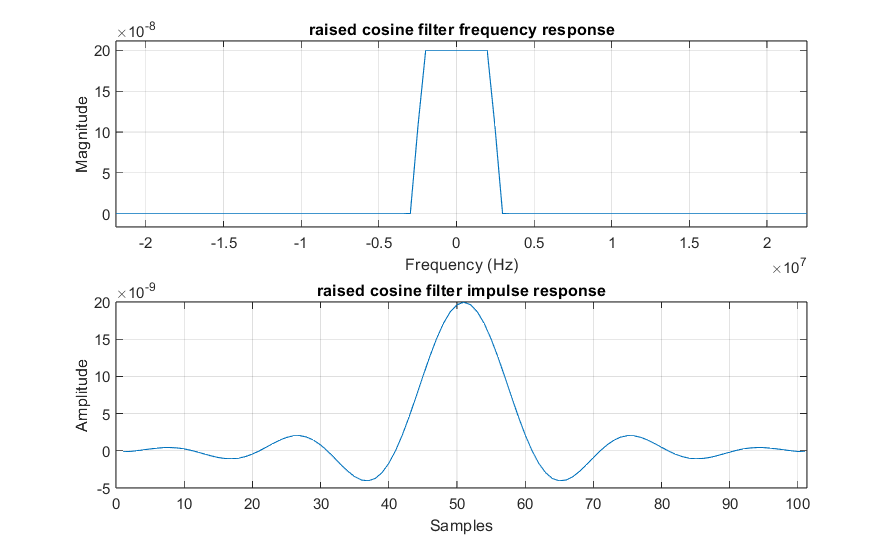
\includegraphics[width=0.9\linewidth]{raisedCosine.png}
    \caption{Time and frequency domain representation of the raised cosine filter}
    \label{fig:raisedCosine}
\end{figure}

\begin{figure}[H]
    \centering
    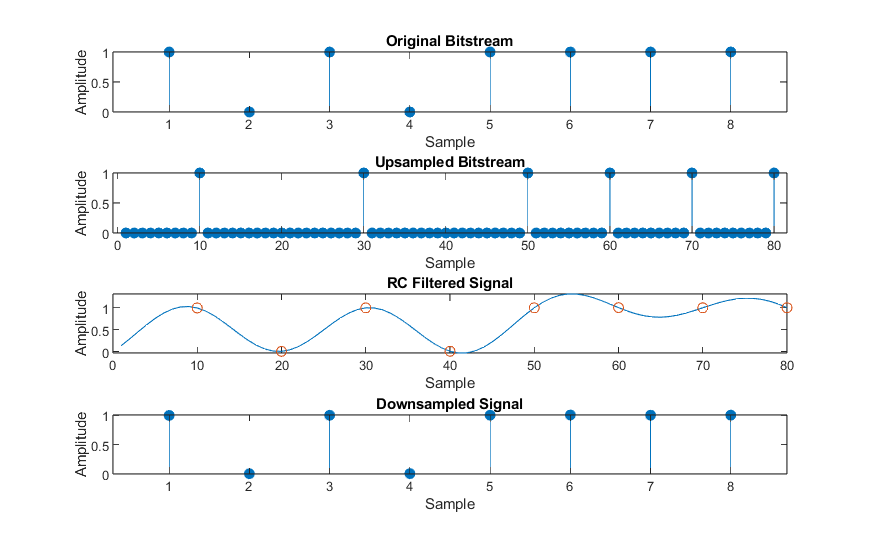
\includegraphics[width=0.9\linewidth]{pulseShaping.png}
    \caption{Pulse shaping with a raised cosine filter}
    \label{fig:pulseShaping}
\end{figure}

\begin{figure}[H]
    \centering
    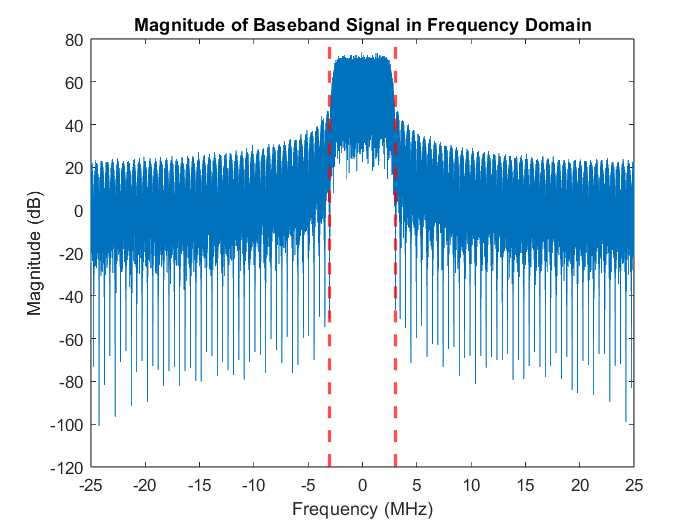
\includegraphics[width=0.9\linewidth]{shapedSpectrum.png}
    \caption{Spectrum of the transmitted signal after pulse shaping}
    \label{fig:shapedSpectrum}
\end{figure}

\section{Noise addition}

The last building block is a noise source. It generates additive white Gaussian noise in baseband. When the signal is corrupted too much, the demodulation can fail. The BER curves are plotted in figure \ref{fig:BER} and they show the impact of the noise power $N_0$ on the bit error rate. The compromise between reliability and capacity is again visible: in the same conditions (same $E_b/N_0$), a modulation with lower capacity will have a smaller BER. \\

The theoretical BER curves are plotted on figure \ref{fig:BER} and are compared with the simulation results. They stay close to each other untill the BER reaches $10^{-4}$. This limit could go even lower by increasing the number of bits sent but we limited it to $10^6$ in order for the code to run quite fast. \\

To impose a value of $E_b/N_0$, we start by computing the energy of the transmitted signal before adding the noise. The power of the noise is then chosen as $N_0 = E_b / (E_b/N_0)_{\text{desired}}$. \\

\begin{figure}[H]
    \centering
    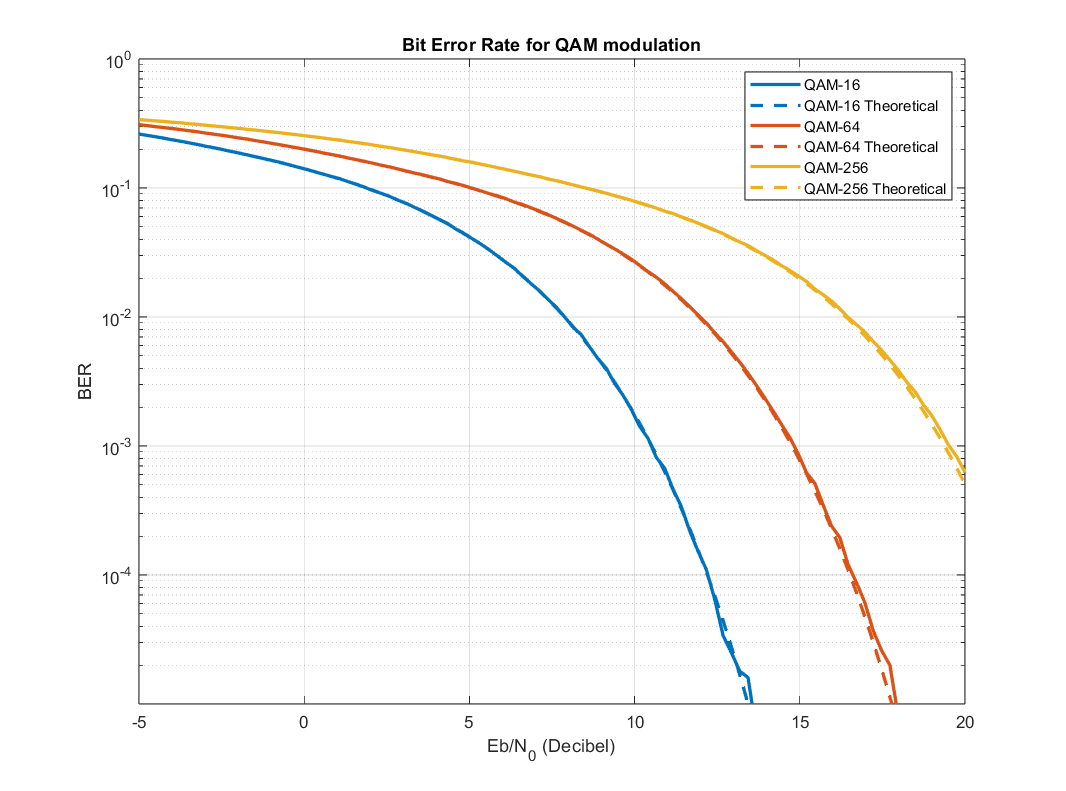
\includegraphics[width=0.9\linewidth]{BERcurve.png}
    \caption{BER curves for different QAM modulations}
    \label{fig:BER}
\end{figure}

\section{Bit rate}

Considering the following characteristics :

    \begin{itemize}
        \item (a) Physical bandwidth of 6 MHz
        \item (b) Roll-off factor = 0.2 
        \item (c) QAM 16 modulation 
    \end{itemize}

We can derive the symbol rate from the physical bandwidth

\begin{equation*}
    f_{symbol} = \frac{B_{physical}}{roll-off-factor} = 5 MHz
\end{equation*}

\begin{equation*}
    Bit-rate = Symbol-rate * Bits-per-symbol = 5MHz*4 = 20 MBps
\end{equation*}

